%ch.tex


\chapter{Parsing requests, monadically}
\begin{center}
{\small\em How to get from the obligatory to the well formed}
\end{center}

\begin{figure}[tbp]
\begin{center}
{ 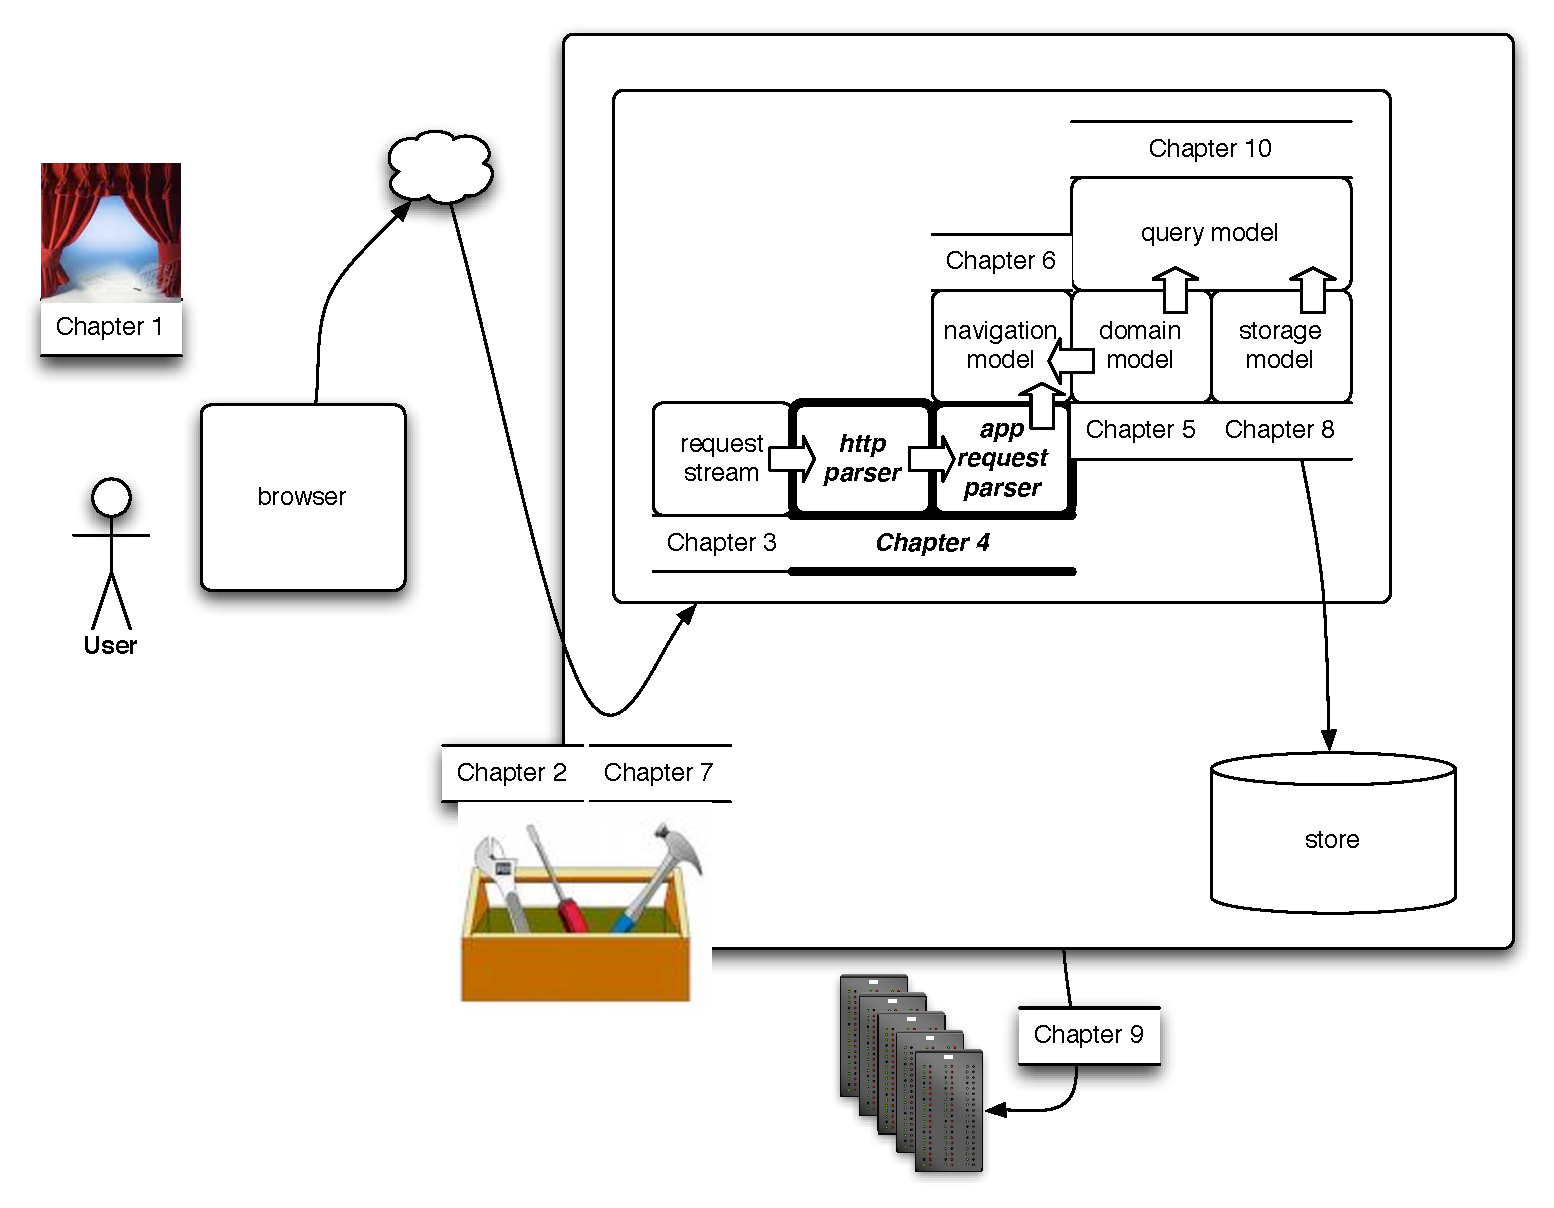
\includegraphics[scale=.35]{/Users/lgm/work/src/projex/biosimilarity/trace/src/main/book/content/figures/MonadicDesignPatternsChapterMapFocus4.pdf} }
\caption{ Chapter map }
\end{center}
\end{figure}

TBD
\section{Obligatory parsing monad}

TDB
\section{Your parser combinators are showing}

TBD
\section{EBNF and why higher levels of abstraction are better}

TBD

% \section{Existence problems}
% We begin with some metamathematics.
% All problems about the existence of maps can be cast into one of the
% following two forms, which are in a sense mutually dual.

% \noindent
% {\bf The Extension Problem}\index{extension problem} \    %%% NB index entry tag
% Given an inclusion $ A \stackrel{i}{\hookrightarrow} X $, and a map
% $ A \stackrel{f}{\rightarrow} Y $,
% does there exist a map $f^{\dagger}:X\to Y$ such that
% $f^{\dagger}$ agrees with $f$ on $A$?

% Here the appropriate source category for maps should be clear from the
% context and, moreover, commutativity through a
% candidate $f^{\dagger}$ is precisely
% the restriction requirement; that is,
% $$f^{\dagger}   :  f^{\dagger}\circ i = f^{\dagger}|_A = f\,. $$
% If such an $f^{\dagger}$ exists\footnote{${}^{\dagger}$ suggests striving
% for perfection, crusading}, then it is called an {\bf
% extension}\index{extension!of a map|bi} of $f$ and is said to {\bf
% extend}\index{extend|bi} $f$. In any diagrams, the presence of
% a dotted arrow or an arrow carrying a ? indicates a pious hope, in no way
% begging the question of its existence. Note that we shall usually
% omit $\circ$ from composite maps.

% \noindent
% {\bf The Lifting Problem}\index{lifting problem} \
% Given a pair of maps $E \stackrel{p}{\rightarrow}B$ and $X \stackrel{f}
% {\rightarrow} B $,
% does there exist a map $f^{\circ} : X \to E$, with
% $pf^{\circ} = f  $?


% That {\em all\/} existence problems about maps are essentially of one
% type or
% the other from these two is seen as follows. Evidently, all existence problems
% are representable by triangular diagrams\index{triangular diagrams} and it
% is easily seen that there are only these six possibilities:
% \begin{center}\begin{picture}(300,70)  %augch2 75
% \put(5,60){\vector(1,0){30}}
% \put(55,60){\vector(1,0){30}}
% \put(135,60){\vector(-1,0){30}}
% \put(185,60){\vector(-1,0){30}}
% \put(235,60){\vector(-1,0){30}}
% \put(285,60){\vector(-1,0){30}}
% \put(0,55){\vector(0,-1){30}}
% \put(50,55){\vector(0,-1){30}}
% \put(100,25){\vector(0,1){30}}
% \put(150,25){\vector(0,1){30}}
% \put(200,55){\vector(0,-1){30}}
% \put(250,55){\vector(0,-1){30}}
% \put(28,33){\small ?}
% \put(78,33){\small ?}
% \put(128,33){\small ?}
% \put(178,33){\small ?}
% \put(228,33){\small ?}
% \put(278,33){\small ?}
% \put(10,3){\bf 1}
% \put(60,3){\bf 2}
% \put(110,3){\bf 3}
% \put(160,3){\bf 4}
% \put(210,3){\bf 5}
% \put(260,3){\bf 6}
% \put(35,55){\vector(-1,-1){30}}
% \put(155,25){\vector(1,1){30}}
% \put(135,55){\vector(-1,-1){30}}
% \put(55,25){\vector(1,1){30}}
% \put(235,55){\vector(-1,-1){30}}
% \put(255,25){\vector(1,1){30}}
% \end{picture}\end{center}



% \begin{figure}
% \begin{picture}(300,220)(0,0)
% \put(-20,-20){\resizebox{20 cm}{!}{\includegraphics{3dpdf}}}
% \put(260,-10){\resizebox{15 cm}{!}{\includegraphics{contpdf}}}
% \put(220,80){$\beta$}
% \put(400,-10){$N$}
% \put(260,170){$\beta$}
% \put(90,15){$N$}
% \end{picture}
% \caption{{\em The log-gamma family of densities with central mean
% $<N> \, = \frac{1}{2}$ as a surface and as a contour plot. }}
% \label{pdf}
% \end{figure}

\newpage
